
\chapter{A NetGen-compatible map browser}

This chapter will present two evolutions of the initial Netgen program for 
support of precise geographic positions and map browsing, then for displaying 
buildings or obstacles representations extracted from OpenStreetMap databases. 
The present tools allow to interact with the more common public information systems 
such as Google map and OpenStreetMap. 

The map browser is a tool allowing to display various kind of maps and to represent 
locations of interest such as sensors set in the country. 
As this tool is developped on the same platform as NetGen, the procedures described 
in chapter \ref{sec:chapter1} will apply to access the software: 
\begin{itemize}
\item start a fresh image and ensure that the NetGen package is loaded with one of the last 
version (1.28.1.2.5 should work)
\item open the store dialog from VisualWorks main window
\item select GoogleMap package (we need to change this name)
\item select version 1.15.5.2 or later, and type load from the pop-up menu
\end{itemize}

The initial window displays as show figure \ref{fig:initialGmap}. 

\begin{figure}
\begin{center} 
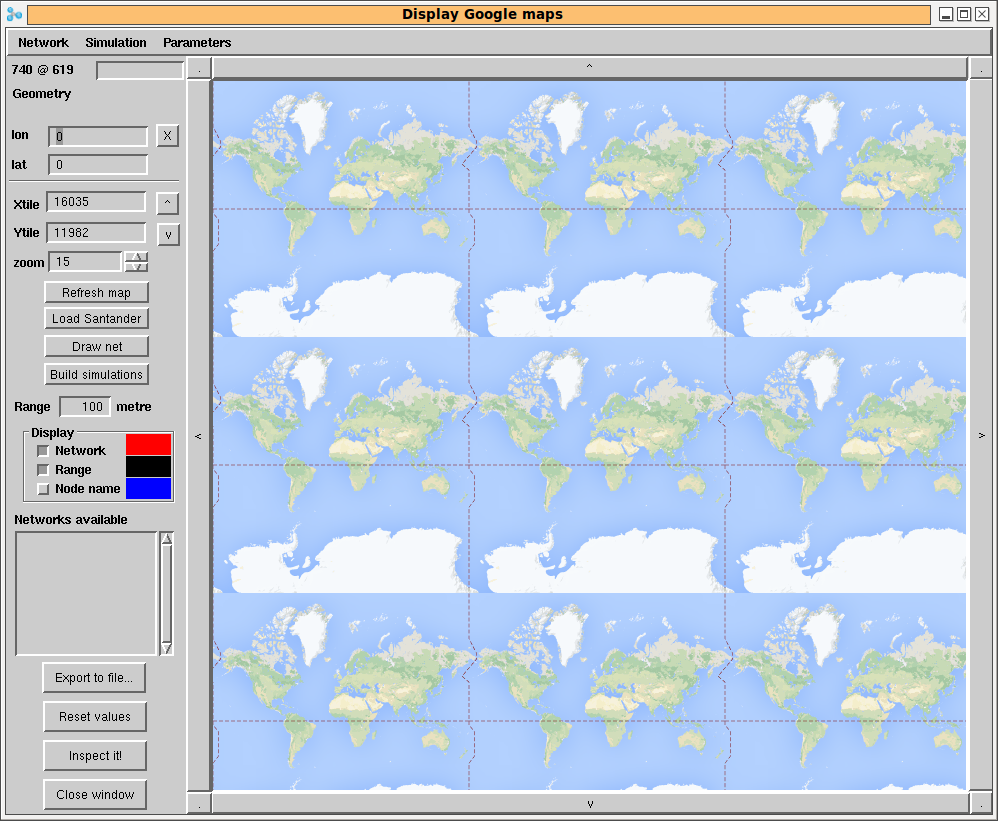
\includegraphics[width=8cm]{gmap.png}
\caption{Initial view on the map browser: the right part displays tiles from the map 
from public servers. The left column displays geographic information and allows 
to control network presentation. }
\label{fig:initialGmap}
\end{center}
\end{figure}

\section{Moving on the map}
A predefined position is visible inside the xtile and ytile fields 
in the left column of the browser. Just below, a zoom factor is also provided. 
Whatever are these values, by pushing the refresh map button, the browser 
will download geographic information to be presented in the graphic pane. 

All around this pane, four sidebars allow to move the graphics top, down, left, and right. 
The four rectangles at the corner of this view control moves on diagonal directions. 

By changing the zoom factor, the absolute view size will decrease or increase. 
As an example going from 15 to 16 increase the level of details. 

\section{Loading networks}
Networks are loaded from external files (further versions will allow direct 
selection from the interface). 

Currently, GPX file format is used, as it is a very common way to describe set of 
points featured with attributes. 

\subsection{Scenario for loading informations}
Suppose that by moving on the map, we have reached a particular region 
where a sensor network is setup or planned.

\begin{figure}
\begin{center}
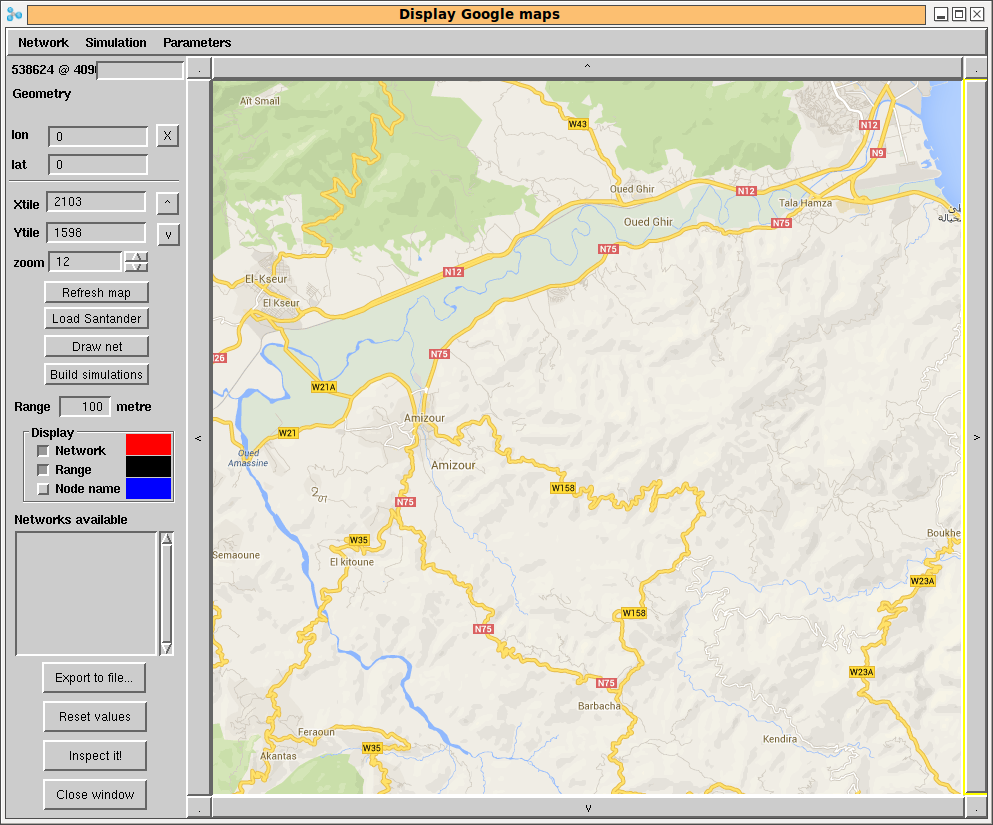
\includegraphics[width=8cm]{soummam0.png}
\caption{The browser is pointing to a North Africa river where sensors are to be installed
for water observations.}
\label{fig:initialSoummam}
\end{center}
\end{figure}


First, let us comments what is a GPX file. In this format, we find a header 
that keep information about the initial source of contents. As an example, 
a header from the Santander website could contain: 

\begin{lstlisting}
<?xml version="1.0" encoding="utf-8"?>
<gpx version="1.0" creator="NetGen for Santander">
  <metadata>
  <name>SmartSantander's sensors</name>
     <desc>Sensors in city: Santander, Spain</desc>
     <link>http://smartsantander.eu/</link>
     <time>2013-06-13T17:45:10</time>
</metadata>
\end{lstlisting}

After this there is a list of entries for each of the location documented by the file. 
In the case of our river, we will find tens of similar entries such as: 

\begin{lstlisting}
<wpt lat="36.679926936710501" lon="4.911090436802451">
  <name>H1-2</name>
  <sym>El Kseur</sym>
</wpt>
<wpt lat="36.682937769536323" lon="4.919011088180600">
  <name>I2</name>
  <sym>El Kseur</sym>
</wpt>
<wpt lat="36.686345105073165" lon="4.929854203839318">
  <name>J3</name>
  <sym>El Kseur</sym>
</wpt>
...
\end{lstlisting}

This a very short information since no practical values appear from sensors. 
The file extraction presents three waypoints (from the initial purpose of the NMEA standard for
GPS), with geographic coordinates as decimal expression of degrees. 
Following we find a name for this particular point, and a symbol to display. 

\subsection{Loading a network}

By using the \emph{Network} menu at top-left we can select the 
\emph{Load Gpx} function that brings a dialog 
to select a GPX file. In our case, it is \emph{soummam.gpx} 
file to remember the name of the river and the file format. 
The file is parsed and its contents appears as points on the graphic part.

The symbols appearing in the entries of the file are used to group waypoints together 
inside networks. This networks are shown in a list in the left column. 
They are selectable, and as an example, the network \emph{El Kseur} is validated 
for display figure \ref{fig:soummam1}. 

\begin{figure}
\begin{center}
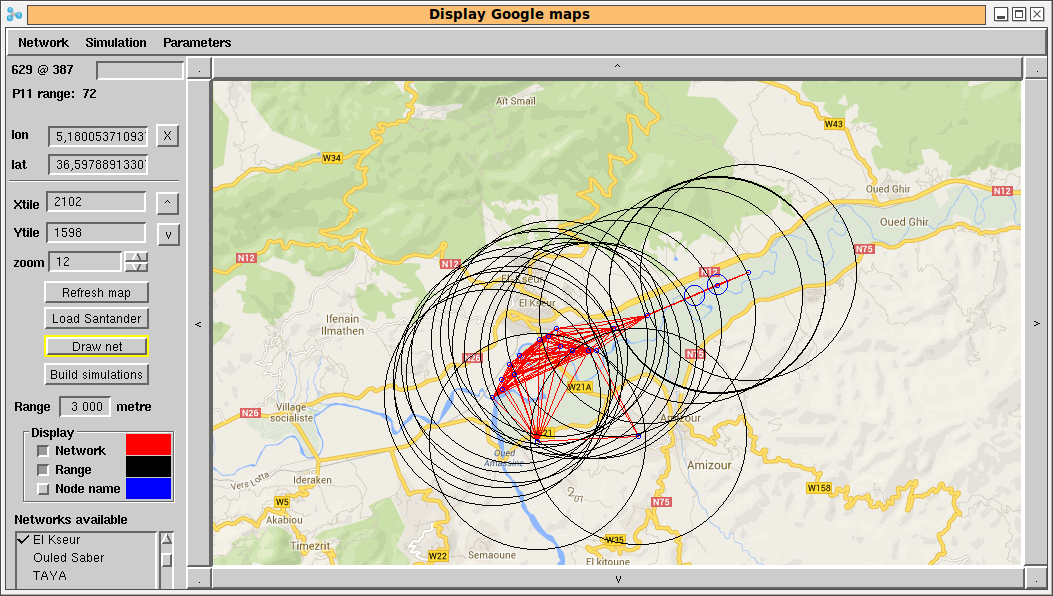
\includegraphics[width=8cm]{soummam1.png}
\caption{The browser is pointing to a North Africa river where sensors are to be installed
for water observations.}
\label{fig:soummam1}
\end{center}
\end{figure}

\subsection{Network configuration}

Several of the functions of NetGen as described in the previous chapter are avalaible from 
this front-end window which capabilities exceed the picking tool shown 
chapter \ref{sec:chapter2}. As an example, the range used to decide wether a sensor 
is connected to another can be defined using a dedicated numeric field. Furthermore, 
the present tool has precise knowledge about geographical points and related distances 
including display distances. Thus, the distance can be defined as meters conforming to 
radio capability specification. 

On figure \ref{fig:soummam1}, the range has been tuned to the point where each sensor 
in the El Kseur network was reachable, giving a necessary range of 3~000 meters to include 
all the sensors. The window does not react directly to range modification, 
it is necessary to call \emph{Draw net} button. 

Some colouring functions ease the display of sensor names, range circles, and connectivities. 

The mouse location over a graphic presentation is tracked on the top-left 
of the window: 

\begin{itemize}
\item point coordinates inside the window, changing to red when the mouse is precisely over 
  a sensor. 
\item this case the logical name of the node is shown in the edit field.
\item a second line presents the range and position of the closest sensor, 
or a communication channel in the case where the mouse is over such a channel.
\end{itemize}


\subsection{Network generation}

To reach Netgen functionalities related to the process graph specification, 
it is sufficient to depress the build simulations button: the specification is 
loaded in every Netgen window (chapter \ref{sec:chapter2} and figure \ref{fig:soummamNetgen})  
for further use: building simulation, graph drawing (see figure \ref{fig:soummamGraph}), etc... 


\begin{figure}
\begin{center}
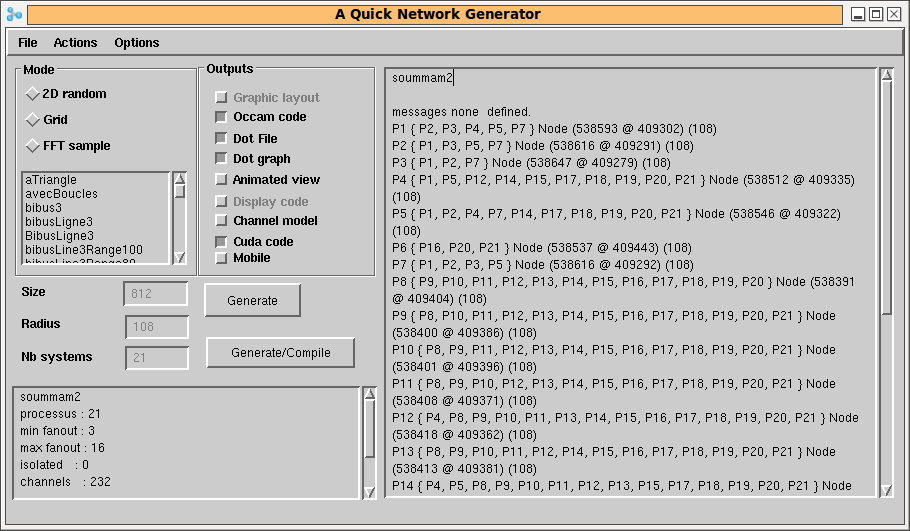
\includegraphics[width=8cm]{netgenSoummam.png}
\caption{Netgen window with El Kseur specification and statistic. }
\label{fig:soummamNetgen}
\end{center}
\end{figure}

\begin{figure}
\begin{center}
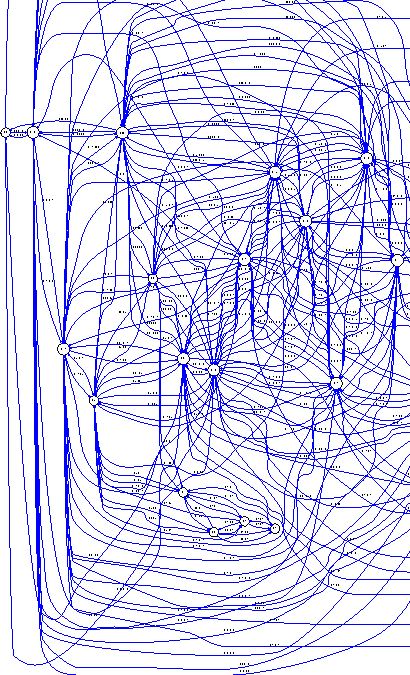
\includegraphics[width=8cm]{soummam2.pdf}
\caption{Logic graph for El Kseur location network.}
\label{fig:soummamGraph}
\end{center}
\end{figure}



After this exploration we have learned that this network has 21 nodes with maximum 
connectivity of 16, with 232 communications channels.

Executing the simulation brings a value of 4 hops for the network diameter. 
We probably have interest to reduce the general range keeping the further nodes to 
a 3~000 m range. 

\section{Loading building architectures}

The package concerned with building representations is MapAccess one, also available from 
the same store server as for chapter \ref{sec:chapter1}. 

In addition to this package, we need some files in the format of "shapefile". This time, 
we propose to do our scenario on the case of Brest city which administration decided 
to produce large description as 80~000 buildings set. 

\begin{itemize}
\item start a fresh image and ensure that the NetGen package is loaded with one of the last
version (1.28.1.2.5 should work)
\item open the store dialog from VisualWorks main window
\item select MapAccess package (in the future, likely to be merged with the map browser)
\item select version 1.6 or later, and type load from the pop-up menu
\item open a system browser, look for the MapAccess package, and the comments 
for this package. It is a button in the middle of the browser window. 
This comment looks like the following sentences:
\\
\emph{Display maps from tile servers, like Google Map or OpenStreetMap.
Georeference points on the map.
Display objects from shapefiles. 
Library is located here: http://wsn.univ-brest.fr/MapAccess/library/libShapeFile.tar. Run 'make' to compile it. 
BMO shapefile is located here: http://wsn.univ-brest.fr/MapAccess/bmo/. Copy the two files shp and shx in the same directory. 
}

This comment is likely to change, but we will keep location allowing to download 
software for the package: dynamic libraries compiled for Linux and MacOSX, and 
shapefiles for Brest. We do not support Window currently. 

\item in your working directory, download the libraries: \\
\verb!wget http://wsn.univ-brest.fr/MapAccess/library/libShapeFile.tar!. 
\\
Desarchive the tar file by doing tar xf libShapeFile.tar. 
\item and download the two shapefiles: 
\\
\verb!wget http://wsn.univ-brest.fr/MapAccess/bmo/bati-WGS84.shp! 
\\ and \\ 
\verb!wget http://wsn.univ-brest.fr/MapAccess/bmo/bati-WGS84.shx!. 
\\
(ftp, curl, or any web browser can do similar work)
\end{itemize}

\subsection{Checking the configuration}

To check the installation, it is best to open a system browser on class 
ShapefileReader (figure \ref{fig:configBrowserShp}). 
This class uses directly the public domain library 
for assessing file conforming to the shapefile format. 
It translates external definitions into objects to be displayed 
on a derivative of the map browser interface. 

\begin{figure}
\begin{center}
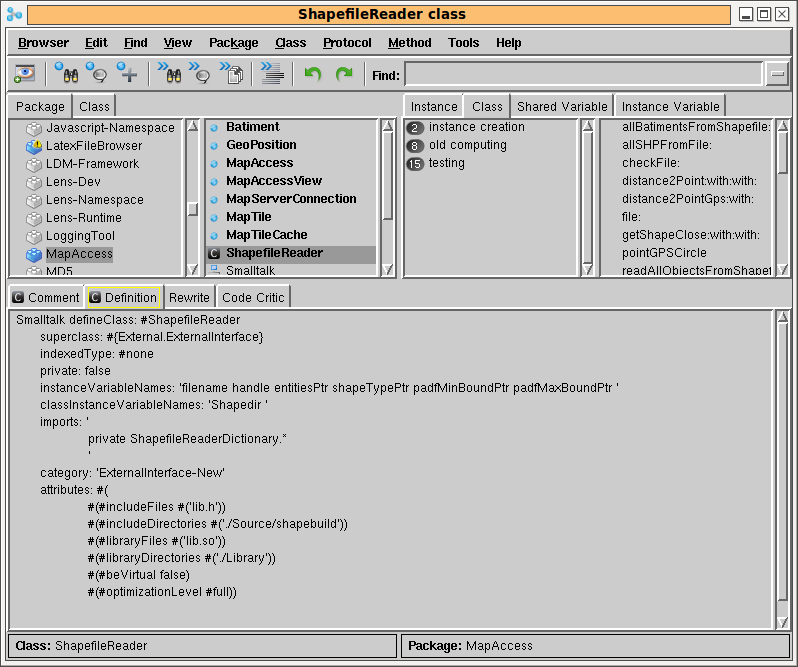
\includegraphics[width=8cm]{config-browser-shp.png}
\caption{Path configuration for the dynamic libraries}
\label{fig:configBrowserShp}
\end{center}
\end{figure}

It can be necessary to adapt the two directories for includeDirectories, 
for libraryDirectories to the platform, observing that a regeneration can be 
possible based on this public software. 


\subsection{Interface opening}
By selecting the Tools menu from the main window, then choosing "Universite... MapAccess"
the new interface opens. This interface is quite similar to the map navigation interface, at 
the exception at the left column. Having the interface open, by clicking 
Reset values, then Refresh map, we obtain a default view on Brest city 
(figure \ref{fig:mapAccessMainWindow}). 

\begin{figure}
\begin{center}
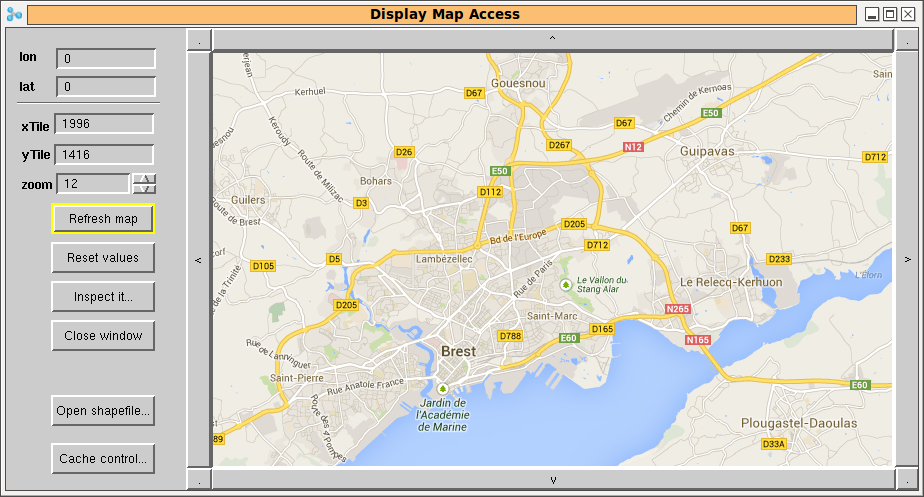
\includegraphics[width=10cm]{mapAccessWindow.png}
\caption{Brest presentation before loading a shapefile}
\label{fig:mapAccessMainWindow}
\end{center}
\end{figure}

\subsection{Loading shapefile}

The button Open shapefile brings a dialog where a .shx file must be selected 
The figure \ref{fig:mapAccessFilled} shows Brest city map with 
more than 80~000 buildings represented as polyline 2D objects. 

\begin{figure}
\begin{center}
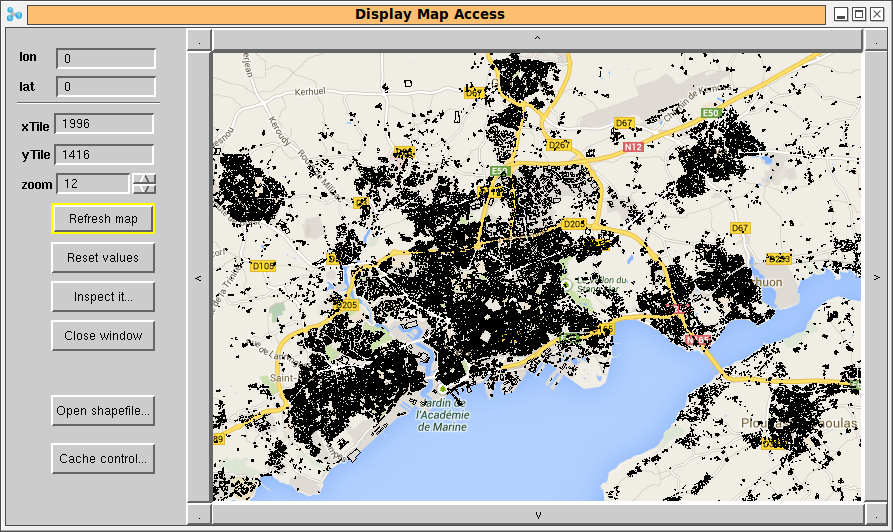
\includegraphics[width=10cm]{mapAccessFilled.png}
\caption{Brest presentation once the shapefile is loaded}
\label{fig:mapAccessFilled}
\end{center}
\end{figure}

\subsection{Browsing the city}

The capabilities of the map browser exists in this preliminary tool. 
As exemple, one can zoom and move the display view changing the level 
of details. The geographic coordinates being preserved, it is possible 
to focus very precise situations to enable simulations and computations. 
See figures \ref{fig:mapAccessGMap} and \ref{fig:mapAccessOSM}. 

\begin{figure}
\begin{center}
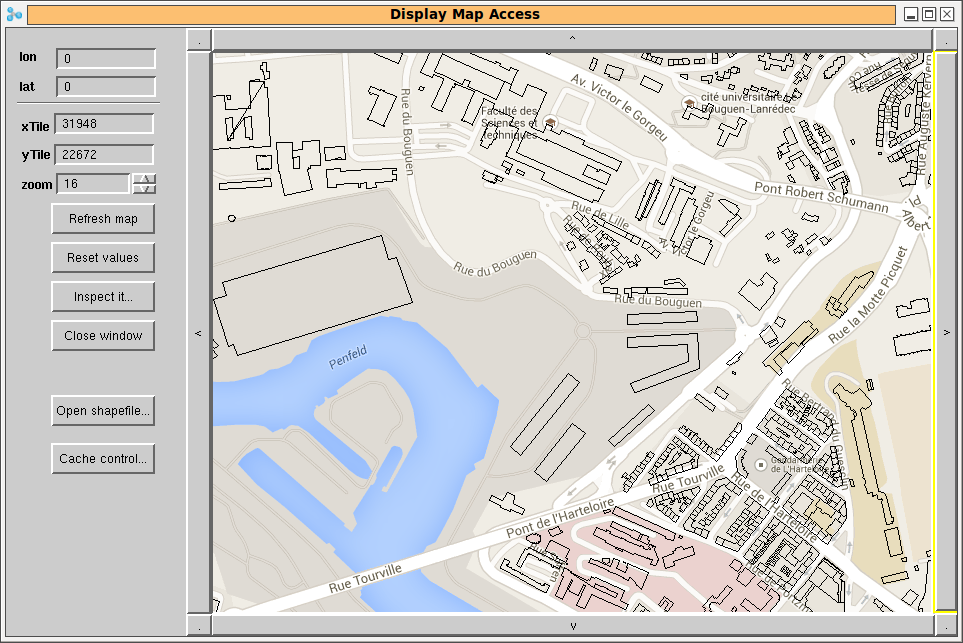
\includegraphics[width=10cm]{mapAccessPenfeldGMap.png}
\caption{Brest university and river Penfeld after loading BMO shapefile, 
Google Maps}
\label{fig:mapAccessGMap}
\end{center}
\end{figure}

\begin{figure}
\begin{center}
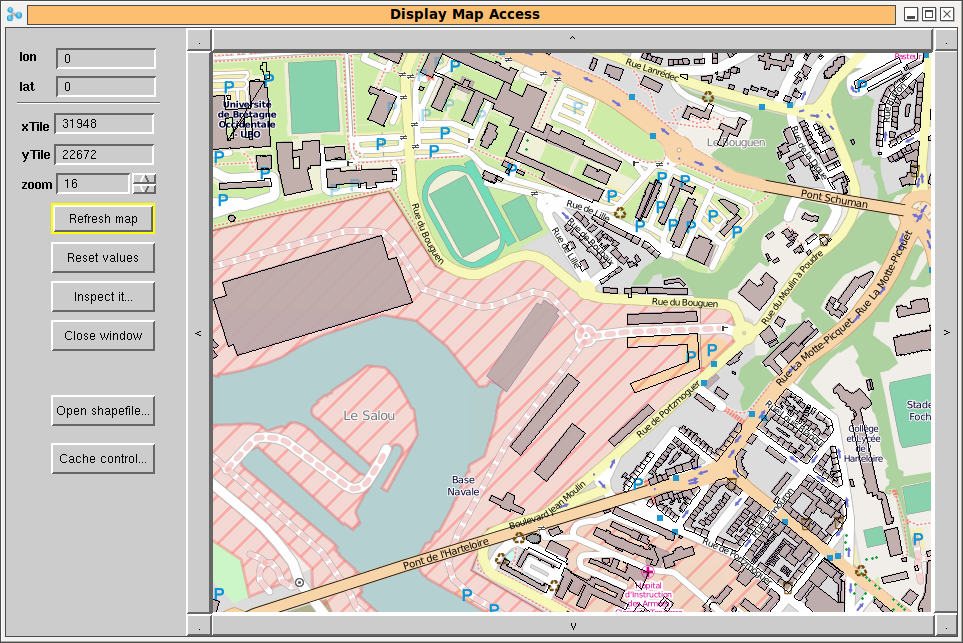
\includegraphics[width=10cm]{mapAccessPenfeldOSM.png}
\caption{The same view as for figure \ref{fig:mapAccessGMap}, using OpenStreetMap.}
\label{fig:mapAccessOSM}
\end{center}
\end{figure}

Switching between map layout is possible using a dialog installed 
under the cache control button. This dialog also allows to empty a cache 
used in the present software to speed up access to distant map tiles. 


